\documentclass[portrait,a4paper]{article}


\usepackage[utf8x]{inputenc}
\usepackage[T1]{fontenc}


\usepackage{mathtools}
\usepackage{amssymb,amsfonts,amsmath}
\usepackage[e]{esvect}

\usepackage{algorithmic}
\usepackage{algorithm}
\newcommand{\algorithmlabel}[2]{{
    \renewcommand{\algorithmicensure}{\textbf{#1}:}
    \ENSURE{#2~}
}}

\usepackage{graphicx}
\usepackage[svgnames]{xcolor}

\usepackage{geometry}
\geometry{a4paper}

% multirow and multicol
\usepackage{multirow}
\usepackage{multicol}
\columnsep24pt
\columnseprule0.1pt

% enumerate
\renewcommand\theenumi{\arabic{enumi}}
\renewcommand\labelenumi{\theenumi.}
\renewcommand\theenumii{\roman{enumii}}
\renewcommand\labelenumii{\theenumii)}

\usepackage{listings}
\lstset{
    floatplacement={tbp},
    basicstyle=\ttfamily\mdseries,
    identifierstyle=,
    stringstyle=\color{gray},
    numbers=left,
    numbersep=5pt,
    inputencoding=utf8x,
    xleftmargin=8pt,
    xrightmargin=8pt,
    keywordstyle=[1]\bfseries,
    keywordstyle=[2]\bfseries,
    keywordstyle=[3]\bfseries,
    keywordstyle=[4]\bfseries,
    numberstyle=\tiny,
    stepnumber=1,
    breaklines=true,
    frame=lines,
    showstringspaces=false,
    tabsize=2,
    commentstyle=\color{gray},
    captionpos=b,
    float=float,
    language={Java}
}
\newcommand{\code}[1]{\lstinline{#1}}

% hyperref
\usepackage[colorlinks=true,pdfborder={0 0 0},citecolor=DarkGreen,linkcolor=DarkBlue,urlcolor=DarkBlue]{hyperref}

% depth of section numbering
\setcounter{secnumdepth}{4}

% redefine the \paragraph command:
\makeatletter
\renewcommand\paragraph{\@startsection{paragraph}{4}{0mm}%
    {-\baselineskip}%
    {0.5\baselineskip}%
    {\normalfont\bfseries}%
}%
\makeatother

% new chapter command
\newcommand{\newchapter}{\clearpage\pagebreak}

% theorems
\usepackage{amsthm}
\newtheorem{lemma}{Lemma}[section]
\newtheorem{theorem}{Theorem}[section]
\newtheorem{corollary}{Corollary}[section]
\newtheorem{definition}{Definition}[section]
\newtheorem{remark}{Remark}[section]
\newtheorem{observation}{Observation}[section]
\newtheorem{assumption}{Assumption}[section]
\newtheorem{proposition}{Proposition}[section]

% autoref names
\newcommand{\specialref}[2]{\hyperref[#1]{#2~\ref*{#1}}}
\def\lstlistingautorefname{Listing}
\def\subsubsectionautorefname{Section}
\def\subsectionautorefname{Section}
\def\figureautorefname{Figure}

% parindent
\parindent0px
\parskip3pt

% redefine greek letters
\renewcommand{\phi}{\varphi}
\renewcommand{\epsilon}{\varepsilon}

% shortcuts in math mode
% \newcommand{\bs}{\boldsymbol}
\newcommand{\mc}{\mathcal}
\newcommand{\ds}{\displaystyle}
\DeclarePairedDelimiter\absimpl{\lvert}{\rvert}
\DeclarePairedDelimiter\normimpl{\lVert}{\rVert}
\newcommand{\abs}[1]{\absimpl*{#1}}
\newcommand{\norm}[1]{\normimpl*{#1}}
\newcommand{\argmax}{\operatorname*{arg\,max}}
\newcommand{\argmin}{\operatorname*{arg\,min}}

% number sets
\newcommand{\R}{\mathbb{R}}
\newcommand{\Z}{\mathbb{Z}}
\newcommand{\N}{\mathbb{N}}
\newcommand{\Q}{\mathbb{Q}}
\newcommand{\C}{\mathbb{C}}
\newcommand{\F}{\mathbb{F}}
\newcommand{\LL}{\mathcal{L}}
\newcommand{\powerset}{\mathcal P}

% probabilities
\newcommand{\Prob}[1]{\operatorname{Pr}\left[#1\right]}
\newcommand{\Ex}[1]{\mathbb{E}\left[#1\right]}

% misc
\newcommand{\bigO}[1]{\mc O\left(#1\right)} % big-o notation

\newcommand{\nop}[1]{} % temporarily remove from output




% todo
\usepackage{framed}
\newenvironment{todo}
{\color{DarkRed} \begin{leftbar}}
{\end{leftbar}}
\newcommand{\inlinetodo}[1]{{\textcolor{DarkRed}{ [\textbf{TODO}: #1]}}}
\newcommand{\mat}[1]{\bs{#1}}
\newcommand{\ma}{\mat{A}}
\newcommand{\mb}{\mat{B}}
\newcommand{\mx}{\mat{X}}
\newcommand{\mv}{\mat{V}}
\newcommand{\muu}{\mat{U}}
\newcommand{\md}{\mat{D}}
\newcommand{\ms}{\mat{S}}
\newcommand{\mz}{\mat{Z}}

\newcommand{\vx}{\mat{x}}
\newcommand{\va}{\mat{a}}
\newcommand{\vb}{\mat{b}}
\newcommand{\vu}{\mat{u}}
\newcommand{\vz}{\mat{z}}

\newcommand{\rd}{\R^D}
\newcommand{\rr}[2]{\R^{#1 \times #2}}

\usepackage{placeins}

\newcommand*{\titleSW}[3]{\begingroup% Story of Writing
\raggedleft
\vspace*{\baselineskip}
{\Huge\textbf{#1}}\\[0.7\baselineskip]
{\large\textbf{#2}}\\[0.5\baselineskip]
{\small #3}\par
\endgroup}

\begin{document}

 \author{Pascal Spörri\\pascal@spoerri.io}
 \title{HOWTO WRITE FAST NUMERICAL CODE\\ EXERCISE 5}
 \date{\today}
\maketitle

\section{Mini-MMM}
The code of this exercise has been run on an Intel Core i5-3570K CPU and Ubuntu 12.04 with gcc 4.6.3 and the compiler flags: \lstinline{-m64 -march=corei7 -fno-tree-vectorize -O3}. The CPU has a Level 1 cache size of $256$ KB ($4\times 32$ KB data caches and $4\times 32$ KB instruction caches) with $32$ KB L1 data cache available per CPU. The Level 2 cache has a total size of $1$ MB with $256$ KB cache available per CPU. The Level 3 cache has a size of $6$ MB and is shared for all CPUs.

\subsection{Blocking for L1 cache}
The L1 cache can hold $4096$ doubles and has a cache line size of $64$ bytes. Hence we have to optimize the inequality:
\begin{align*}
    \left\lceil {N_B^2 \over B_1} \right\rceil + 3\left\lceil {N_B M_U \over B_1} \right\rceil
    + \left\lceil {N_U M_U \over B_1} \right\rceil \leq {C_1 \over B_1}
\end{align*}


\subsubsection{code1}
$M_U=2$, $N_U=2$, $K_U=1$. The inequality:
\begin{align*}
    \left\lceil {N_B^2 \over 8} \right\rceil + 3\left\lceil {N_B 2 \over 8} \right\rceil
    + \left\lceil {4 \over 8} \right\rceil \leq {4096 \over 8}
\end{align*}
holds an optimal value of $N_B=61$.  Running our code with $N_B=60$ results in a performance of $0.68$ flops/cycle.
\subsubsection{code2}
$M_U=2$, $N_U=2$, $K_U=2$. The inequality:
\begin{align*}
    \left\lceil {N_B^2 \over 8} \right\rceil + 3\left\lceil {N_B 2 \over 8} \right\rceil
    + \left\lceil {4\over 8} \right\rceil \leq {4096 \over 8}
\end{align*}
holds an optimal value of $N_B=61$. Running our code with $N_B=60$ results in a performance of $1.02$ flops/cycle.

\subsubsection{code3}
$M_U=1$, $N_U=8$, $K_U=2$. The inequality:
\begin{align*}
    \left\lceil {N_B^2 \over 8} \right\rceil + 3\left\lceil {N_B \over 8} \right\rceil
    + \left\lceil {8 \over 8} \right\rceil \leq {4096 \over 8}
\end{align*}
holds an optimal value of $N_B=62$. Due to blocking we had to run the code with $N_B=56$ and were able to achieve a performance of $1.30$ flops/cycle.

Thus we are able to conclude that \lstinline{code3.c} performs best for level 1 blocking. This is also supported by the performance plot in figure \ref{fig:flops_cycle}.

\begin{figure}[H]
    \centering
    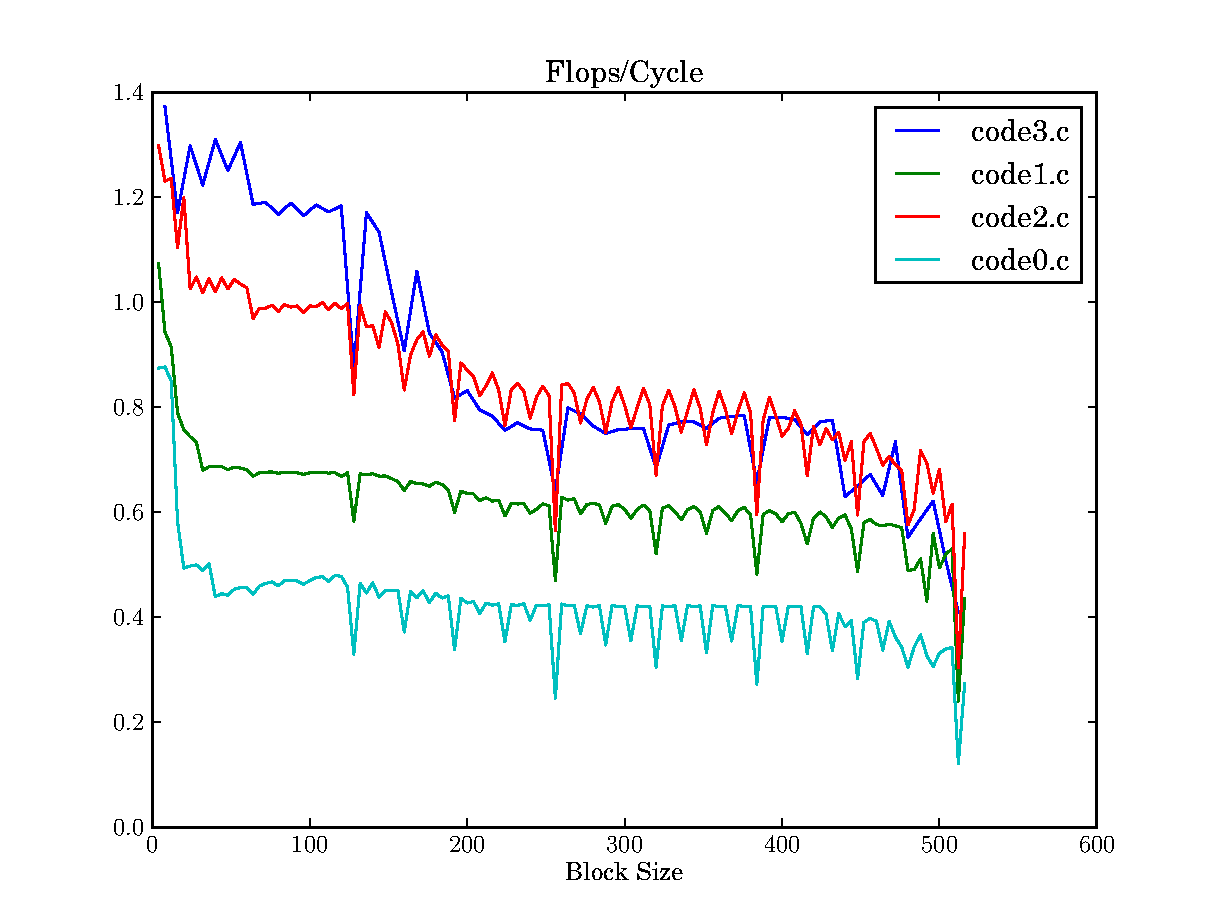
\includegraphics[width=0.9\textwidth]{code/flops_cycle}
    \caption{Performance Plot showing flops/cycle for the different codes. Compiler flags: \texttt{-m64 -march=corei7 -fno-tree-vectorize -O3} (gcc 4.6.3) on an Intel Core i5-3570K CPU.}
    \label{fig:flops_cycle}
\end{figure}  

\subsection{Blocking for L2 cache}
The L1 cache can hold $32768$ doubles and has a cache line size of $512$ bytes. Hence we have to optimize the inequality:

\begin{align*}
    \left\lceil {N_B^2 \over B_1} \right\rceil + 3\left\lceil {N_B M_U \over B_1} \right\rceil
    + \left\lceil {N_U M_U \over B_1} \right\rceil \leq {C_1 \over B_1}
\end{align*}


\subsubsection{code1}
$M_U=2$, $N_U=2$, $K_U=1$. The inequality:
\begin{align*}
    \left\lceil {N_B^2 \over 64} \right\rceil + 3\left\lceil {N_B 2 \over 64} \right\rceil
    + \left\lceil {4 \over 64} \right\rceil \leq {32768 \over 64}
\end{align*}
holds an optimal value of $N_B=177$.  Running our code with $N_B=176$ results in a performance of $0.65$ flops/cycle.
\subsubsection{code2}
$M_U=2$, $N_U=2$, $K_U=2$. The inequality:
\begin{align*}
    \left\lceil {N_B^2 \over 64} \right\rceil + 3\left\lceil {N_B 2 \over 64} \right\rceil
    + \left\lceil {4\over 64} \right\rceil \leq {32768 \over 64}
\end{align*}
holds an optimal value of $N_B=177$. Running our code with $N_B=176$ results in a performance of $0.88$ flops/cycle.

\subsubsection{code3}
$M_U=1$, $N_U=8$, $K_U=2$. The inequality:
\begin{align*}
    \left\lceil {N_B^2 \over 64} \right\rceil + 3\left\lceil {N_B \over 64} \right\rceil
    + \left\lceil {8 \over 64} \right\rceil \leq {32768 \over 64}
\end{align*}
holds an optimal value of $N_B=179$. Due to blocking we had to run the code with $N_B=176$ and were able to achieve a performance of $0.94$ flops/cycle.

Thus we are able to conclude that \lstinline{code3.c} performs best for level 2 blocking. This is also supported by the performance plot in figure \ref{fig:flops_cycle}.

%code3.c
%[(8, 1.372439), (16, 1.170124), (24, 1.298042), (32, 1.223054), (40, 1.309561), (48, 1.250796), (56, 1.304052), (64, 1.186326), (72, 1.190037), (80, 1.167218), (88, 1.18883), (96, 1.164341), (104, 1.185112), (112, 1.171913), (120, 1.183233), (128, 0.873967), (136, 1.170184), (144, 1.133518), (152, 1.018658), (160, 0.907003), (168, 1.058912), (176, 0.941018), (184, 0.905647), (192, 0.817189), (200, 0.831454), (208, 0.794626), (216, 0.78294), (224, 0.755633), (232, 0.770478), (240, 0.758406), (248, 0.756162), (256, 0.640245), (264, 0.798633), (272, 0.787144), (280, 0.764215), (288, 0.749834), (296, 0.757032), (304, 0.758847), (312, 0.758893), (320, 0.684258), (328, 0.765785), (336, 0.771886), (344, 0.77179), (352, 0.759643), (360, 0.778821), (368, 0.782736), (376, 0.783708), (384, 0.657174), (392, 0.780247), (400, 0.780598), (408, 0.776278), (416, 0.747586), (424, 0.771874), (432, 0.775151), (440, 0.629565), (448, 0.649902), (456, 0.67175), (464, 0.631768), (472, 0.734018), (480, 0.552342), (488, 0.587203), (496, 0.620976), (504, 0.508259), (512, 0.408803)]
%code1.c
%[(4, 1.072948), (8, 0.94305), (12, 0.914603), (16, 0.789038), (20, 0.756628), (24, 0.743714), (28, 0.732871), (32, 0.680221), (36, 0.686284), (40, 0.686297), (44, 0.686754), (48, 0.680854), (52, 0.685793), (56, 0.68399), (60, 0.680918), (64, 0.66832), (68, 0.674716), (72, 0.676237), (76, 0.676529), (80, 0.673952), (84, 0.675856), (88, 0.675786), (92, 0.674828), (96, 0.671962), (100, 0.675006), (104, 0.67508), (108, 0.675778), (112, 0.674254), (116, 0.675333), (120, 0.667812), (124, 0.675065), (128, 0.582613), (132, 0.672958), (136, 0.67118), (140, 0.673165), (144, 0.668618), (148, 0.668847), (152, 0.663932), (156, 0.658242), (160, 0.641321), (164, 0.658117), (168, 0.654528), (172, 0.653634), (176, 0.649421), (180, 0.65684), (184, 0.652661), (188, 0.641916), (192, 0.599853), (196, 0.639769), (200, 0.635863), (204, 0.634593), (208, 0.622247), (212, 0.627463), (216, 0.621096), (220, 0.622431), (224, 0.592656), (228, 0.616111), (232, 0.615522), (236, 0.615673), (240, 0.597892), (244, 0.605481), (248, 0.615492), (252, 0.612222), (256, 0.47), (260, 0.628775), (264, 0.622855), (268, 0.625618), (272, 0.596783), (276, 0.614376), (280, 0.617019), (284, 0.613758), (288, 0.578376), (292, 0.611183), (296, 0.614187), (300, 0.605383), (304, 0.588468), (308, 0.605293), (312, 0.613568), (316, 0.602584), (320, 0.52082), (324, 0.607491), (328, 0.612304), (332, 0.601134), (336, 0.585162), (340, 0.604869), (344, 0.610726), (348, 0.600684), (352, 0.559714), (356, 0.602991), (360, 0.610659), (364, 0.598122), (368, 0.583543), (372, 0.603164), (376, 0.608724), (380, 0.594988), (384, 0.481426), (388, 0.596021), (392, 0.602494), (396, 0.596957), (400, 0.581554), (404, 0.596584), (408, 0.600094), (412, 0.578923), (416, 0.539409), (420, 0.588624), (424, 0.600466), (428, 0.590831), (432, 0.57106), (436, 0.588842), (440, 0.594641), (444, 0.568288), (448, 0.486937), (452, 0.579793), (456, 0.586082), (460, 0.576236), (464, 0.573828), (468, 0.577353), (472, 0.573983), (476, 0.57052), (480, 0.489242), (484, 0.490432), (488, 0.51107), (492, 0.430656), (496, 0.559722), (500, 0.493669), (504, 0.519362), (508, 0.530441), (512, 0.240071), (516, 0.43575)]
%code2.c
%[(4, 1.297601), (8, 1.230612), (12, 1.235551), (16, 1.103185), (20, 1.199148), (24, 1.025189), (28, 1.047832), (32, 1.018026), (36, 1.044286), (40, 1.020251), (44, 1.046107), (48, 1.025345), (52, 1.043067), (56, 1.034572), (60, 1.027498), (64, 0.968794), (68, 0.98809), (72, 0.988681), (76, 0.993709), (80, 0.982315), (84, 0.995308), (88, 0.990448), (92, 0.992877), (96, 0.979582), (100, 0.993048), (104, 0.990836), (108, 0.999622), (112, 0.985369), (116, 0.998086), (120, 0.987572), (124, 0.997165), (128, 0.823854), (132, 0.994212), (136, 0.953359), (140, 0.95497), (144, 0.913993), (148, 0.981411), (152, 0.960765), (156, 0.919782), (160, 0.83268), (164, 0.899377), (168, 0.928359), (172, 0.943079), (176, 0.896987), (180, 0.937696), (184, 0.918805), (188, 0.906876), (192, 0.774328), (196, 0.883981), (200, 0.870965), (204, 0.858784), (208, 0.821486), (212, 0.840962), (216, 0.865073), (220, 0.832736), (224, 0.764349), (228, 0.833187), (232, 0.845181), (236, 0.829863), (240, 0.778722), (244, 0.81881), (248, 0.84004), (252, 0.821652), (256, 0.564535), (260, 0.841812), (264, 0.845077), (268, 0.826892), (272, 0.769787), (276, 0.814477), (280, 0.837906), (284, 0.810367), (288, 0.751617), (292, 0.809678), (296, 0.837628), (300, 0.803649), (304, 0.760374), (308, 0.799163), (312, 0.835749), (316, 0.8051), (320, 0.670132), (324, 0.802451), (328, 0.832357), (332, 0.800795), (336, 0.752442), (340, 0.792813), (344, 0.832837), (348, 0.798028), (352, 0.72808), (356, 0.789408), (360, 0.829956), (364, 0.796803), (368, 0.749035), (372, 0.792068), (376, 0.827372), (380, 0.788753), (384, 0.595295), (388, 0.775536), (392, 0.818705), (396, 0.783816), (400, 0.744944), (404, 0.759145), (408, 0.793086), (412, 0.767353), (416, 0.669166), (420, 0.763286), (424, 0.727938), (428, 0.758854), (432, 0.737614), (436, 0.752285), (440, 0.698935), (444, 0.734267), (448, 0.594552), (452, 0.733899), (456, 0.750092), (460, 0.7209), (464, 0.68948), (468, 0.705879), (472, 0.6902), (476, 0.679188), (480, 0.575644), (484, 0.605512), (488, 0.717044), (492, 0.693344), (496, 0.635618), (500, 0.681838), (504, 0.581483), (508, 0.614905), (512, 0.304138), (516, 0.558837)]
%code0.c
%[(4, 0.874371), (8, 0.87663), (12, 0.849749), (16, 0.581496), (20, 0.493401), (24, 0.497226), (28, 0.499349), (32, 0.488972), (36, 0.502254), (40, 0.439002), (44, 0.444706), (48, 0.441584), (52, 0.452981), (56, 0.456421), (60, 0.456669), (64, 0.443232), (68, 0.459338), (72, 0.46418), (76, 0.467058), (80, 0.459245), (84, 0.470048), (88, 0.470188), (92, 0.468919), (96, 0.462853), (100, 0.469399), (104, 0.475411), (108, 0.477022), (112, 0.468286), (116, 0.479119), (120, 0.477829), (124, 0.456961), (128, 0.329401), (132, 0.464069), (136, 0.445879), (140, 0.465246), (144, 0.437936), (148, 0.450402), (152, 0.450634), (156, 0.450411), (160, 0.371621), (164, 0.448952), (168, 0.436868), (172, 0.449798), (176, 0.427867), (180, 0.445371), (184, 0.436424), (188, 0.440375), (192, 0.33783), (196, 0.436053), (200, 0.42686), (204, 0.429847), (208, 0.407052), (212, 0.42682), (216, 0.422948), (220, 0.425334), (224, 0.353171), (228, 0.423397), (232, 0.422521), (236, 0.425643), (240, 0.393935), (244, 0.422976), (248, 0.421569), (252, 0.423371), (256, 0.245637), (260, 0.425034), (264, 0.421426), (268, 0.422697), (272, 0.36836), (276, 0.421932), (280, 0.419144), (284, 0.421723), (288, 0.346904), (292, 0.422544), (296, 0.419653), (300, 0.42041), (304, 0.354982), (308, 0.42154), (312, 0.41945), (316, 0.420461), (320, 0.304396), (324, 0.421537), (328, 0.419438), (332, 0.421967), (336, 0.354895), (340, 0.422426), (344, 0.419721), (348, 0.421708), (352, 0.332276), (356, 0.422029), (360, 0.420067), (364, 0.420795), (368, 0.354577), (372, 0.421526), (376, 0.420766), (380, 0.420777), (384, 0.27217), (388, 0.420619), (392, 0.420521), (396, 0.420695), (400, 0.353974), (404, 0.420589), (408, 0.420193), (412, 0.420345), (416, 0.330341), (420, 0.419415), (424, 0.420659), (428, 0.4052), (432, 0.335703), (436, 0.406811), (440, 0.381807), (444, 0.394172), (448, 0.283555), (452, 0.390012), (456, 0.397713), (460, 0.39188), (464, 0.336926), (468, 0.391994), (472, 0.361985), (476, 0.342762), (480, 0.304915), (484, 0.343408), (488, 0.366122), (492, 0.32656), (496, 0.305655), (500, 0.331654), (504, 0.339164), (508, 0.342069), (512, 0.12099), (516, 0.272752)]


\end{document}